%%%%%%%%%%%%%%%%%%%%%%%%%%%%%%%%%%%%%%%%%%%%%%%%%%%%%%%%%%%%%%%%%%%%%%%%%%%%%%%%%
%
% Purpose:  Verification part of V&V for the ThermalRider model
%
% 
%
%%%%%%%%%%%%%%%%%%%%%%%%%%%%%%%%%%%%%%%%%%%%%%%%%%%%%%%%%%%%%%%%%%%%%%%%%%%%%%%%

% \section{Verification}

%%% code imported from old template structure
%\inspection{<Name of Inspection>}\label{inspect:<label>}
% <description> to satisfy  
% requirement \ref{reqt:<label>}.
\subsection{Inspections}

\inspection{Top-level Inspection}\label{inspect:top_level}
This document, the code, and associated files, have been inspected, and together
satisfy requirement~\ref{reqt:top_level}.

\inspection{Extended Functionality} \label{inspect:thermal_ext_func}
The method \textit{ThermalFacetRider::accumulate\_thermal\_sources} includes the
functionality to add thermal power sources or sinks (see \textref{Verification
of Intra-vehicular Thermal Transfer}{test:intravehicularthermaltransfer}), and a good description of how a conduction model could be implemented.  The addition of heating due to aerodynamic drag has not been investigated in depth, but it is anticipated that this would be handled by the aerodynamics model by adding a Thermal Rider to the existing aerodynamics model.  This satisfies requirement~\ref{reqt:thermal_ext_func}



\subsection{Verification of the Temperature Modeling}
\label{test:temperature}

  The simulations for this verification procedure are found in the Radiation Pressure model; this verification test is duplicated in the Radiation Pressure model.
  
  This section is divided into two parts, one comparing the case of
  the vehicle without illumination --- for which an analytic solution
  exists --- and the second comparing the response of surfaces with different
  characteristics in the presence of illumination.

  \subsubsection{Verification of thermal processes without illumination}
  \test{Thermal Processes - no illumination}
  \label{test:temperature_integration1}
  \begin{description}
  \item{Purpose:}\ \newline
    This test is to ensure that the Runge-Kutte plate-temperature integration
    process is functioning normally in the case of a vehicle cooling in the
    absence of incident radiation.
  \item{Requirements:}\ \newline
    Satisfactory conclusion of this test, along with test~\ref{test:temperature_integration2} satisfies requirements~\ref{reqt:temp_monitoring} and~\ref{reqt:thermal_min_func}.
  \item{Procedure:}\ \newline
    The simulation used in this test is available at \newline
    \textit{radiation\_pressure/verif/SIM\_2\_SHADOW\_CALC/RUN\_shadow\_cooling}.
    A number of facets were monitored in a flux-free environment to observe
    their temperature variation with time.  Each plate had
    slightly different characteristics, allowing for the dependency on
    emissivity, plate area, and heat capacity to be investigated.  In the
    absence of incident flux, an analytic solution exists for the temperature
    and the force, and this can be compared to the numerical solution.
  \item{Results:}
    \begin{enumerate}
    \item{Variation with time of temperature}\newline
      Simulation data of the variation with time of temperature matched very well to analytic solution.  On any scale
      longer than 3 timesteps, the graphs of analytical values and simulation
      values were indistinguishable, with a difference less than 0.05\%, and
      very much smaller than the observed changes in temperature.  See Figure~\ref{fig:temperatureanalytic}.
      \begin{figure}[!ht]
         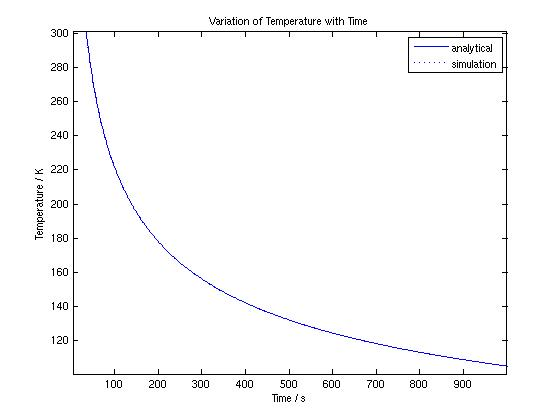
\includegraphics[width=180mm]{figures/temperature_analytic.jpg}
         \caption{Variation of Temperature with time showing the simulation data
         and analytic solution overlaying.}
         \label{fig:temperatureanalytic}
      \end{figure}
    \item{Variation with emissivity of the temporal evolution of temperature}\newline
      As the emissivity increases, the rate of change of temperature also
      increases, as expected.  For $\epsilon$=0, no temperature
      change was observed.
    \item{Variation with starting temperature of the temporal evolution of temperature}\newline
      With a lower starting temperature, a plate maintains a lower temperature
      throughout the simulation, but the temperature decreases more slowly.
      Temperature$\sim$time plots have identical shapes; shifting the curves along
      the x-axis to match temperature at some time results in matching
      temperatures for all (valid) time.
    \item{Variation with plate area of the temporal evolution of temperature}\newline
      A plate with a smaller surface area, but identical heat capacity shows a
      more gradual temperature drop.  There is no observable difference between
      plates for which the heat capacity is decreased proportionally with the 
      area (e.g. smaller plate of the same material). 
    \item{Variation with heat capacity of the temporal evolution of temperature}\newline
      A plate with a smaller heat capacity, but identical area shows a
      more rapid temperature drop.  There is no observable difference between
      plates for which the area is decreased proportionally with the heat 
      capacity (e.g. smaller plate of the same material). 
    \end{enumerate}
    
  \end{description}
  \clearpage

  \subsubsection{Verification of thermal processes with illumination}
  \test{Thermal Processes - with illumination}
  \label{test:temperature_integration2}
  \begin{description}
  \item{Purpose:}\ \newline
    To verify that the temperature integration and thermal emission processes
    are functioning as expected when the vehicle is illuminated.
  \item{Requirements:}\ \newline
    Satisfactory conclusion of this test, along with test~\ref{test:temperature_integration1} satisfies requirements~\ref{reqt:temp_monitoring} and~\ref{reqt:thermal_min_func}.
    
  \item{Procedure:}\ \newline
  The simulation used in this test is available at \textit{SIM\_2\_SHADOW\_CALC/RUN\_ten\_plates}.
    10 identical plates were oriented at different angles to the flux
    vector, with the angle between the normal and the flux vector varying
    from 0 to 90 degrees.  All plates were started with a preliminary
    temperature of 270 K, and the simulation was allowed to run until all but
    one plate had approached their equilibrium temperature.  The force from each plate
    was monitored throughout the simulation. 
  \item{Results:}\ \newline
    The equilibrium temperature is calculated from the energy balance equation
    \begin{equation}
      \phi (A\cos \theta )(1-\alpha )=\epsilon \sigma A{T_{\mathit{eq}}}^{4}
    \end{equation}
        
    where
    \begin{itemize}
      \item{} 
        $\phi$ is the radiative flux, 
      \item{} 
        $\theta$ is the angle between the surface normal and the incident
        radiation vector, 
      \item{}
        $\alpha$ is the albedo of the surface, 
      \item{}
        $\epsilon$ is the emissivity of the surface, 
      \item{}
        $\sigma$ is the Stefan-Boltzmann constant, 
      \item{}
        A is the plate area, and
      \item{}  
        $T_{\mathit{eq}}$ is the equilibrium temperature.
    \end{itemize}

    Using values of $\alpha =0.5$,  $\epsilon =0.5$, $\phi =
    1400~W~ m^{-2}$, and with $\theta$ varying from 0 to 90 degrees in 10 degree 
    intervals, the equilibrium temperatures of the 10 plates are:

    396 K, 395 K, 390 K, 382 K, 371 K, 355 K, 333 K, 303 K, 256 K, and 0 K.
    
    Figure~\ref{fig:ivv_F_emission_Tint} shows the variation with time of the
    temperature of the 10 plates; the 9 plates that had closely approached equilibrium temperatures had 
    final temperatures all within
    1\% of their analytical equilibrium temperature.  The final plate, with an equilibrium temperature of 0 K has a temperature
    variation that is decreasing at a rate consistent with expectations.
    
      \begin{figure}[!ht]
        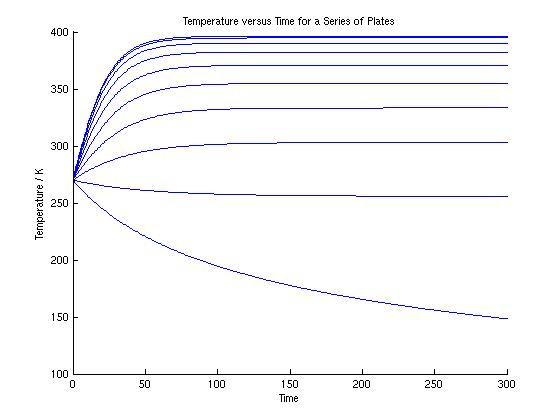
\includegraphics[width=180mm]{figures/temperature-time.jpg}
        \caption{The variation of temperature with time over the 10 plates in
        the simulation.} 
        \label{fig:ivv_F_emission_Tint}
      \end{figure}
  \end{description}
    

    
\clearpage

\test{Verification of Intra-vehicular Thermal Transfer} \label{test:intravehicularthermaltransfer}
\begin{description}
\item{Purpose:}\newline
To test the capability of modeling thermal energy transfer from within the vehicle to the surface.
\item{Requirements:}\newline
Satisfactory conclusion of this test, together with inspection \ref{inspect:thermal_ext_func} satisfies requirement \ref{reqt:thermal_ext_func}
\item{Procedure:}\newline
A test comparable to the basic Radiation Pressure test \newline
(\textit{interactions/radiation\_pressure/verif/SIM\_1\_BASIC/RUN\_basic}) was
performed (at \textit{interactions/radiation\_pressure/verif/SIM\_1\_BASIC/RUN\_thermal\_dump}).  The difference being that in this test, a thermal power dump sufficient to raise the temperature of the surface by 1 degree per second was added.
\item{Predictions:}\newline
The temperature of the surface should initially rise by 1 degree per second above the temperature of the surface without the thermal power input.  As radiative cooling increases in response, the rate of change should diminish over time; eventually a new equilibrium will be reached at some higher temperature than the case with no thermal power dump.
\item{Results:}\newline
The results were as expected; after 1 second, the temperature difference was 0.985 degrees; after 2 seconds, 1.94 degrees (0.97 degrees per second average); after 10 seconds, 8.6 degrees (0.86 degrees per second average); after 25 seconds, 17 degrees (0.68 degrees per second average).

\end{description}
